\section{이론적 배경}

\subsection{천체 관측 시스템}

Fig. \ref{fig:observing_system}\은 관측 환경이 좋은 곳으로 망원경을 이동하여 사진 관측을 할 수 있는 소형 천체 망원경 시스템을 보여 준다. 사진 관측을 위한 천체 망원경 시스템은 크게 광학계(optic), 검출기(detector), 마운트(mount)로 이루어지며, 정밀도를 높이기 위해 가이드 시스템을 포함한 여러가지 보조 도구들이 필요하다. 광학계의 결상 성능, 마운트의 추적 성능 등을 갖추고 있어야 오랜 시간동안 노출을 주며 천체 사진을 찍을 수 있게 된다. 

앞서 제시한 Fig. \ref{fig:The_Andromeda_Galaxy}의 안드로메다 은하 사진은 Fig. \ref{fig:observing_system}\을 이용하여 촬영한 것이다. 상세 정보를 보면 Sbig(Santa Barbara Instrument Group)사의  ST-8300M이라는 모노크롬 CCD(Charge-coupled device)를 이용하여 촬영하였으며, 노출 정보를 보면 L(Luminence) 채널의 경우 600 sec의 노출로 14 frame을 촬영하여 합성하였으며, R(Red), G(Green), B(Blue) 각각의 채널에서 400 sec의 노출로 6 frame씩 촬영하여 합성한 것이다. 이처럼 고품질의 천체사진 한 장을 촬영하기 위해서 많은 시간과 노력이 필요하다. 

\begin{figure}[h]
	\begin{center}
		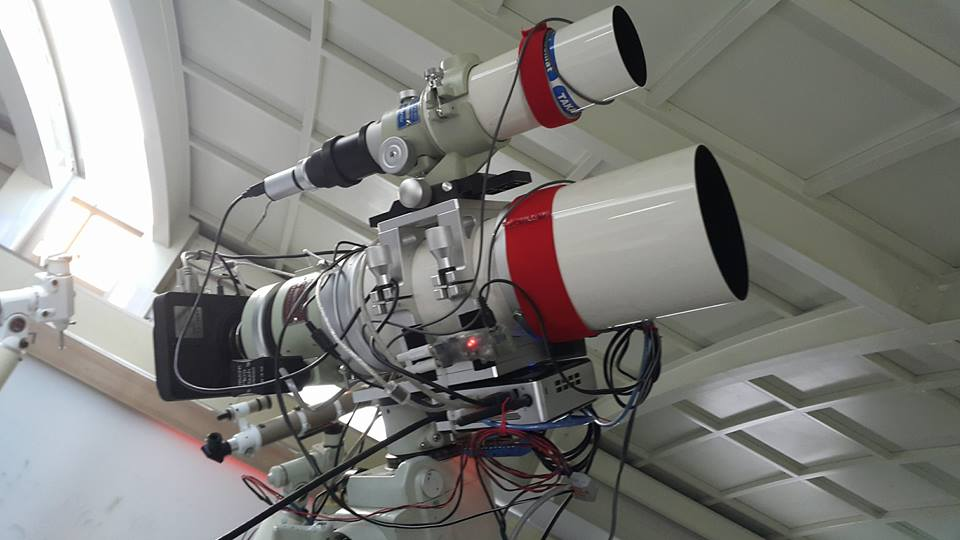
\includegraphics[width=0.9\linewidth]{observing_system}
	\end{center}
		\begin{tikzpicture} [remember picture, overlay]
		\node[rectangle, draw, fill=black!10, minimum size=0.5] at (1.5, 2.5) {(a)};
		\node[rectangle, draw, fill=black!10, minimum size=0.5] at (2.5, 2.5) {(b)};
		\node[rectangle, draw, fill=black!10, minimum size=0.5] at (2.5, 3.5) {(c)};
		\node[rectangle, draw, fill=black!10, minimum size=0.5] at (2.5, 3.5) {(d)};
		\end{tikzpicture}
		\caption{A Small Telescope observing system for astrophotography : (a) main optic, (b) CCD, (c) guide optic, (d) guide CCD}
		\label{fig:observing_system}

\end{figure}

점 광원(Point light source)인 별빛은 대기

\subsection{자동 초점 조절}

이덕규 외(2014)는 복합재 광구조체와 결합하여 전자광학카메라의 영상 품질을 향상시킬 수 있는 초점 조절 장치를 개발하였다.\cite{leedukgu2014}\\
윤종환 외(2011)는 선명도에 관한 기울기를 이용하여 초점이 맞았는지를 확인하는 방법을 사용하였다.\cite{yunjonghwan2011lcd}\\
박석휘 외(2009)는 모바일 폰용 자동 초점 조절 알고리즘을 초점 값 계산 알고리즘을 이용하여 구현하였다.\cite{parksukhui2009Median}\\
이성희 외(1998)는 각 화소들의 미디언 값의 차이를 이용하여 초점을 맞추는 알고리즘을 구현하였다.\cite{leeseonghee1998Median}


\subsection{기존 제품 분석}

Fig. \ref{fig:microtouch}\가 바로 미국의 Starizona사에서 판매하는 Micro Touch  제품이다. Fig. \ref{fig:microtouch_3}\가 Micro Touch Autofocuser Hand Control system (Wired)이고, USB 케이블로 컴퓨터와 연결하여 ASCOM 호환 소프트웨어에서 제어가 가능하다.  Fig. \ref{fig:microtouch_3}\는 Feather touch focuser에 모터를 장착한 모습이다. 

%%%%%%%새로 그림 추가함 (박기현샘)

\begin{figure}[H]
		\begin{subfigure}{0.45\textwidth}
		\begin{center}
			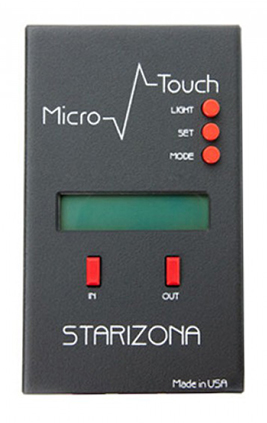
\includegraphics[width=0.6\linewidth]{microtouch_3} 
		\end{center}			
			\caption{Micro touch hand control system (Wired)}
			\label{fig:microtouch_3}
		\end{subfigure}
		\begin{subfigure}{0.45\textwidth}
		\begin{center}			
			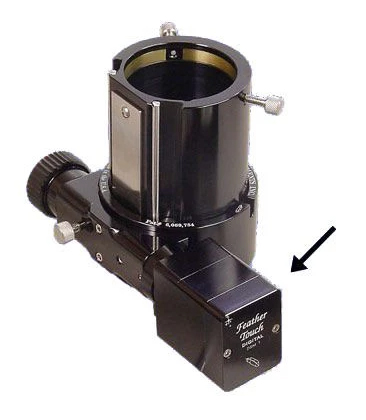
\includegraphics[width=0.75\linewidth]{microtouch_4}
		\end{center}
			\caption{Feather touch focuser with motor}
			\label{fig:microtouch_4}
		\end{subfigure}
		\caption{Starizona사에서 개발하여 판매하는 Micro touch 제품}
		\label{fig:microtouch}
\end{figure}


Fig. \ref{fig:microtouch_3}의 Micro touch 핸드 컨트롤러에 보이는 붉은 색 두 버튼(IN, OUT)은 각각 초점을 맞추기 위해 모터를 정방향, 역방향으로 회전시키는 버튼이다. Micro Touch는 버튼을 눌러 동작시킬 수 있을 뿐 아니라 USB(Universal serial port) 포트를 통해 PC와 연결하여 ASCOM driver 호환 소프트웨어를 통히 모터를 돌려 초점을 조절할 수 있다. 

%를 통해  수동 혹은 자동으로 작동시켜 IN 또는 OUT의 명령을 내렸을 경우, 모터 초점 조절 장치가 작동하게 된다. 이 모터 초점 조절 장치는 모터를 움직여 천체망원경의 경통의 길이를 조절할 수 있도록 한다. 경통의 길이가 변화하면 그에 따라서 빛이 퍼지는 정도가 달라지므로 이를 잘 조정하면 망원경으로 관측하는 천체의 초점을 맞출 수 있다.
하지만 이 제품은 다음과 같은 단점이 있다. 

첫째, Micro Touch 핸트 컨트롤러는 디스플레이를 이용하여 사용하는 사람들이 편하게 사용할 수 있도록 하였다. 2x16 LCD(Liquid-crystal display) displayer를 사용하여 문자 표현이 제한적이어서 여러 상황을 표현하는데 어려움이 있다. 

둘째, 제품의 크기가 매우 커서 한 손으로 잡고 조작하는데 불편하다. 핸드 컨트롤러라고 부르기에 적합하지 않을 정도로 너무 크게 설계되었다. 

셋째, Micro Touch 핸드 컨트롤러는 모터를 조절하는 것에도 한계가 있다. 자신의 회사에서 판매하는 모터를 회전시키는 데는 문제가 없으나 많은 전류를 필요로하는 모터는 탈조가 나서 사용할 수 없다. 또한 microstepping을 바꿀 수 없다. 

\subsection{제품 설계}

기존에 출시되어 있는 모터 포커서 컨트롤러의 장점은 그대로 구현하고, 단점을 보완한 모터 포커서 컨트롤러를 제작하기 위하여 아두이노(Arduino)를 이용하였다. 아두이노는 오픈 소스를 기반으로 한 단일 보드 MCU(MicroController Unit) 보드와 관련 개발 도구 및 환경을 말한다. 2005년 이탈리아의 IDII(Interaction Design Institutelvera)에서 하드웨어에 익숙지 않은 학생들이 자신들의 디자인 작품을 손쉽게 제어할 수 있게 하려고 고안된 아두이노는 처음에 AVR을 기반으로 만들어졌으며, 아트멜 AVR 계열의 보드가 현재 가장 많이 판매되고 있다. ARM 계열의 Cortex-M0(Arduino M0 Pro)과 Cortex-M3(Arduino Due)를 이용한 제품도 존재한다. 현재 출시되어 있는 아두이노 보드 (Arduino board)들을 Table \ref{table:arduino_boards}에 나타내었다. 최근에는 이 보드들과 호환되는 저렴한 아두이노 호환 보드들도 판매되고 있으며, 드라이버만 제대로 설치되면 사용상 큰 문제는 없다. 

% Please add the following required packages to your document preamble:
%https://www.tablesgenerator.com/
% \usepackage{multirow}
\begin{table}[ht]
	\caption{Arduino boards. \cite{wiki-arduino}}
	\begin{tabular}{c|l|l}
	\toprule[1pt]
		& MCU        & Arduino boards                            \\ 
		\toprule[1pt]
	
		\multirow{5}{*}{AVR} & ATmega168  & Pro(168), Mini(168), LilyPad (168V)                                     \\
		& ATmega328  & UNO, Fio, Nano, Pro(328), Mini(328, Rev5, 5V), Pro Mini, LilyPad (328V) \\
		& ATmega2560 & Mega 2560, Mega ADK                                                     \\
		& ATmega32U4 & Yún, Leonardo, Esplora, Micro                                           \\
		& ATtiny85   & GEMMA                                                                   \\ 
		\midrule[1pt]
		\multirow{2}{*}{ARM} & Cortex-M0+ & Zero, Zero PRO, M0, M0 PRO                                              \\
		& Cortex-M3  & Due      \\
	\bottomrule[1pt]   
	\end{tabular}
	\label{table:arduino_boards}
\end{table}

아두이노는 다수의 스위치나 센서로부터 값을 받아들여, LED나 모터와 같은 외부 전자 장치들을 통제함으로써 환경과 상호작용이 가능한 물건을 만들어 낼 수 있다. 임베디드 시스템 중의 하나로 쉽게 개발할 수 있는 환경을 이용하여, 장치를 제어할 수 있다. 아두이노 통합 개발 환경(IDE)을 제공하며, 소프트웨어 개발과 실행코드 업로드도 제공한다 \cite{wiki-arduino}. 

포커서를 구동하기 위한 모터는 스테핑 모터 (spetting motor)를 사용하였다. 선풍기와 같이 우리가 실생활에서 볼 수 있는 모터는 대부분 DC 모터(direct current motor)이다. DC 모터는 전류가 흐르는 상태일 때 코일에 의해 계속 회전하는 원리를 사용하고 있기 때문에 원하는 위치나 각도에서 정지시키는 것이 어렵다. 때문에 망원경의 초점을 조절할 때에는 DC 모터를 사용하는 경우 정밀하게 회전을 제어하는데 어려움이 따른다. 

스테핑 모터의 여러 가지 특성은 정밀하게 제어해야 하는 포커서에 적합하다. 스테핑 모터는 그 상세한 종류에 따라 모양은 다르게 생겼지만 대부분의 스테핑 모터를 차지하는 PM형 모터의 경우 회전축에는 영구자석이 붙어있어 회전자(rotor)를 이루고, 바깥쪽에는 일정한 각도로 부착되어있는 전자석이 존재하여 고정자(Stator)를 이루게 된다. 외부에서 각 선에 전류를 흘려보내면, 전자석이 작동하여 회전자를 움직이게 만드는 원리로 움직인다. 쉽게 말하자면 '전류펄스로 제어되는 움직임'이 DC 모터와 비교했을 때 스테핑 모터의 가장 큰 특징이다. 때문에 고정자들은 그 사이의 각도가 일정한 성질과 더해 한번 펄스를 쏠 때마다 일정한 각도를 움직이게 되며, 같은 양의 펄스를 주면 항상 같은 거리를 이동하므로 정확한 거리 계산에 용이하다.

또한 모터에 펄스형태가 아닌 선형으로 전류를 가하게 되면 안쪽의 회전자는 그대로 고정되어 힘을 받게 된다. 이 때 받는 힘의 크기를 홀적 토크라고 하며, 펄스 형태의 전류가 가해지지 않으면 모터는 움직이지 않고 정지한 상태를 유지한다. 이를 이용한 스테핑 모터의 또다른 특징이 바로 microstepping이다. 대부분의 스테핑 모터는 고정자의 전자석이 배치된 개수가 200개로 고정이 되어있어 한번 펄스를 가할 때 360/200인 1.8도(이를 single step, 혹은 full step이라 한다)를 움직이게 된다. 하지만 가하는 총 전류에 비해 약한 전류변화를 일으키면 full step에 비해 적은 각도 변화를 일으키게 되고, 이를 여러 단계로 나눈 것이 microstepping이다. 이를 활용하면 망원경의 특성에 따라 적절하게 모터의 힘과 속도, 위치의 정확성을 개선할 수 있다.

microstepping 뿐만 아니라 모터의 정확성과 힘에 관여하는 요소는 많이 존재한다. 대체적으로  모터에 가해지는 전류펄스의 크기가 커지게 되기 때문에 전압에 비례해 토크가 커지게 된다. 또한, 모터의 속도는 가한 총 펄스에 비례하기 때문에 속도가 빨라지게 되면 가하는 펄스의 관성에 약해지게 되고 탈조현상이 일어날 가능성이 커지게 되며, 모터의 토크도 약해지게 된다. 비슷한 원리로, 전류펄스의 크기를 약하게 만드는 microstepping또한 모터의 토크를 저하시키게 된다.

\subsubsection{Visual Studio 및 ASCOM standard}
Visual Studio는 Microsoft에서 제공하는 통합 개발 환경으로, Visual Basic, Visual C\# 등 여러 가지 언어를 제공하며, Windows .NET환경에서 개발을 진행할 수 있다는 큰 장점이 있다. 본 드라이버의 언어 또한 Windows. NET을 기반으로 하고 있으므로 Windows. NET 기반의 개발 환경을 제공하는 Visual Studio를 사용하면 개발이 크게 편리해진다. 추후 개발이 원활하게 진행되면, MFC 라이브러리를 이용한 드라이버의 개발을 진행하여 개발의 직관성을 더 높일 수도 있을 것이며, MFC 라이브러리를 이용하며 만든 드라이버 또한 Visual Studio를 통한 원활한 개발이 가능하다. 이를 위해서는 C\#으로 개발된 프로그램을 regasm.exe로 활성화시킬 필요가 있다.

ASCOM standard는 망원경을 움직이기 위하여 지원하는 시스템 중 하나로, 현재 제작되고 사용되는 많은 망원경들이 ASCOM standard를 따르고 있기 때문에 이를 사용하여 망원경을 움직이는 프로그램을 만들게 되면 여러 망원경에도 같이 사용할 수 있게 되어 호환성에 있어 큰 이점을 가지게 된다. 이것이 가능한 이유는 ASCOM standard 만의 신호 (protocol)이 존재하기 때문인데, 드리아버를 사용하여 이를 펌웨어와 연결시켜 통신을 할 때, ASCOM standard protocol을 사용하면 펌웨어와의 통신이 원활하게 이루어질 수 있게 되고, 다른 드라이버와도 연결할 수 있게 만들 수 있게 된다.

ASCOM은 Visual Studio를 이용한 여러 가지 예제나 개발 환경을 제공하는데, developer 버전을 제공하여 아이콘이나, 실행 배경 등 Visual Studio를 이용한 ASCOM 드라이버의 개발에 필요한 여러 작업 환경들을 지원한다.
